\subsection{Overview}

One known fact about human decision-making is that context can affect people's choices. That is, the relative likelihood of choosing one option over another can vary systematically with the menu of options, the \textit{choice set}. These findings are known as \textit{context effects}. One notable context effect, the attraction effect, occurs when the choice share of a \textit{target} option is boosted upon the inclusion of a similar but inferior \textit{decoy} option. Another finding, the repulsion effect, occurs when a decoy boosts the choice share of a \textit{dissimilar} option, known as the \textit{competitor}, rather than the target.

The attraction and repulsion effects, originally studied in preferential choice, have recently been shown to occur in simple perceptual decision-making \parencite{trueblood2013not,spektorWhenGoodLooks2018b}. This is theoretically interesting because it suggests that context effects are a theoretical primitive rather than a feature of high-level choice \parencite{trueblood2013not}. The goal of this research is to understand how and why these effects occur by employing well-studied statistical models from the psychology and economics literature. 

This dissertation is structured as follows. In Chapter 1, I introduce the relevant empirical and theoretical literature in context effects. The goal of Chapter 2 is to develop and test a statistical model of perceptual variability when applied to context effects. In Experiment 1, I first show that the types of stimuli used in perceptual choice context effects experiments are easily confusable and vary systematically with theoretically relevant properties of the stimuli. In Experiment 2, I use the results of a high-powered psychophysics experiment to show that the repulsion effect, but not the attraction effect, is naturally predicted by this statistical model due to the fact that pairs of similar stimuli are more strongly perceptually correlated than pairs of dissimilar stimuli. In Chapter 3, I further test the statistical model by applying it to best-worst choice. In Chapter 4, I generalize the model to preferential choice. 

\subsection{Introducing the Attraction Effect}

In decision-making experiments, researchers present participants with a finite set of options on each trial and ask them to select a single option. Researchers universally assume that participants use the input they receive (i.e., the value of each option) to arrive at a choice. The study of choice spans multiple fields, including psychology, economics, marketing, and political science. In economics, for example, researchers have developed models based on the idea that, while preferences may vary from moment to moment, people generally make rational choices in any given choice setting \parencite{mcfadden2001economic}. In psychology and marketing, however, researchers have identified a set of phenomena that violate such assumptions, by showing that choices vary based on the \textit{choice set}, or the menu of available options. This class of phenomena is known as \textit{context effects} \parencite{adler2024forty}.

Context effects are interesting to decision-making researchers because they violate properties of large classes of choice models, such as Independence of Irrelevant Alternatives (IIA) \parencite{ray1973independence} and regularity \parencite{mcfadden2001economic}. Psychologists have developed numerous cognitive process models to explain how context effects can arise \parencite{roeMultialternativeDecisionField2001a,usherLossAversionInhibition2004a,truebloodMultiattributeLinearBallistic,wollschlager2NaryChoiceTree2012a,bergnerVAMPVotingAgent2019b,noguchiMultialternativeDecisionSampling2018a,bhatiaAssociationsAccumulationPreference2013b,tversky1993context}. These models vary considerably in their mechanisms but align in the common assumption that decision makers take in the veridical values of each option on each attribute and use these values to arrive at a preference state, leading to a decision. 

This dissertation will explore context effects in both perceptual and preferential decision-making. In particular, I will explore the attraction effect and its reversal, the repulsion effect. I summarize these effects and the relevant literature below.

To begin, I first demonstrate a notable context effect, the \textit{attraction effect}. As a demonstration, see \ref{fig:fig_opts} (left panel), which shows a graphical configuration of various choice options. These options vary on two dimensions (or attributes), where higher values of an attribute are always preferred. I give these dimensions generic names to emphasize that they may be anything from the fuel efficiency and horsepower of cars in a consumer choice experiment to the height and width of rectangles in a perceptual choice experiment.

In Figure \ref{fig:fig_opts} (left panel), options $A$ and $B$ trade off on attributes. $A$ is high on dimension 2 but low on dimension 1, while $B$ is high on dimension 1 but low on dimension 2. A decision-maker who assigns equal importance to both dimensions should be indifferent between both options when presented with choice set $[A,B]$. Now, however, consider option $D_{A}$, which is inferior to $A$ and $B$, but more similar to $A$ than to $B$\footnote{Similarity here is negatively related to distance in attribute space \parencite{shepardUniversalLawGeneralization1987c}.}. Similarly, $D_{B}$ is inferior to both $A$ and $B$ but more similar to $B$. The attraction effect is the finding that choice for $A$ over $B$ is greater given set ${A,B,D_{A}}$ then given set $A,B,D_{B}$\footnote{This is the weak version of the attraction effect. A strong version requires the ordering of P(A) and P(B) to change with choice set. See \textcite{davis2023illustrated} for a discussion of similar issues.}. 
Choice models often, though not necessarily, assume the \textit{Independence of Irrelevant Alternatives}(IIA) principle. IIA states that the relative likelihood of choosing a particular option over another is invariant of the choice set \parencite{ray1973independence}. 

\begin{figure}
   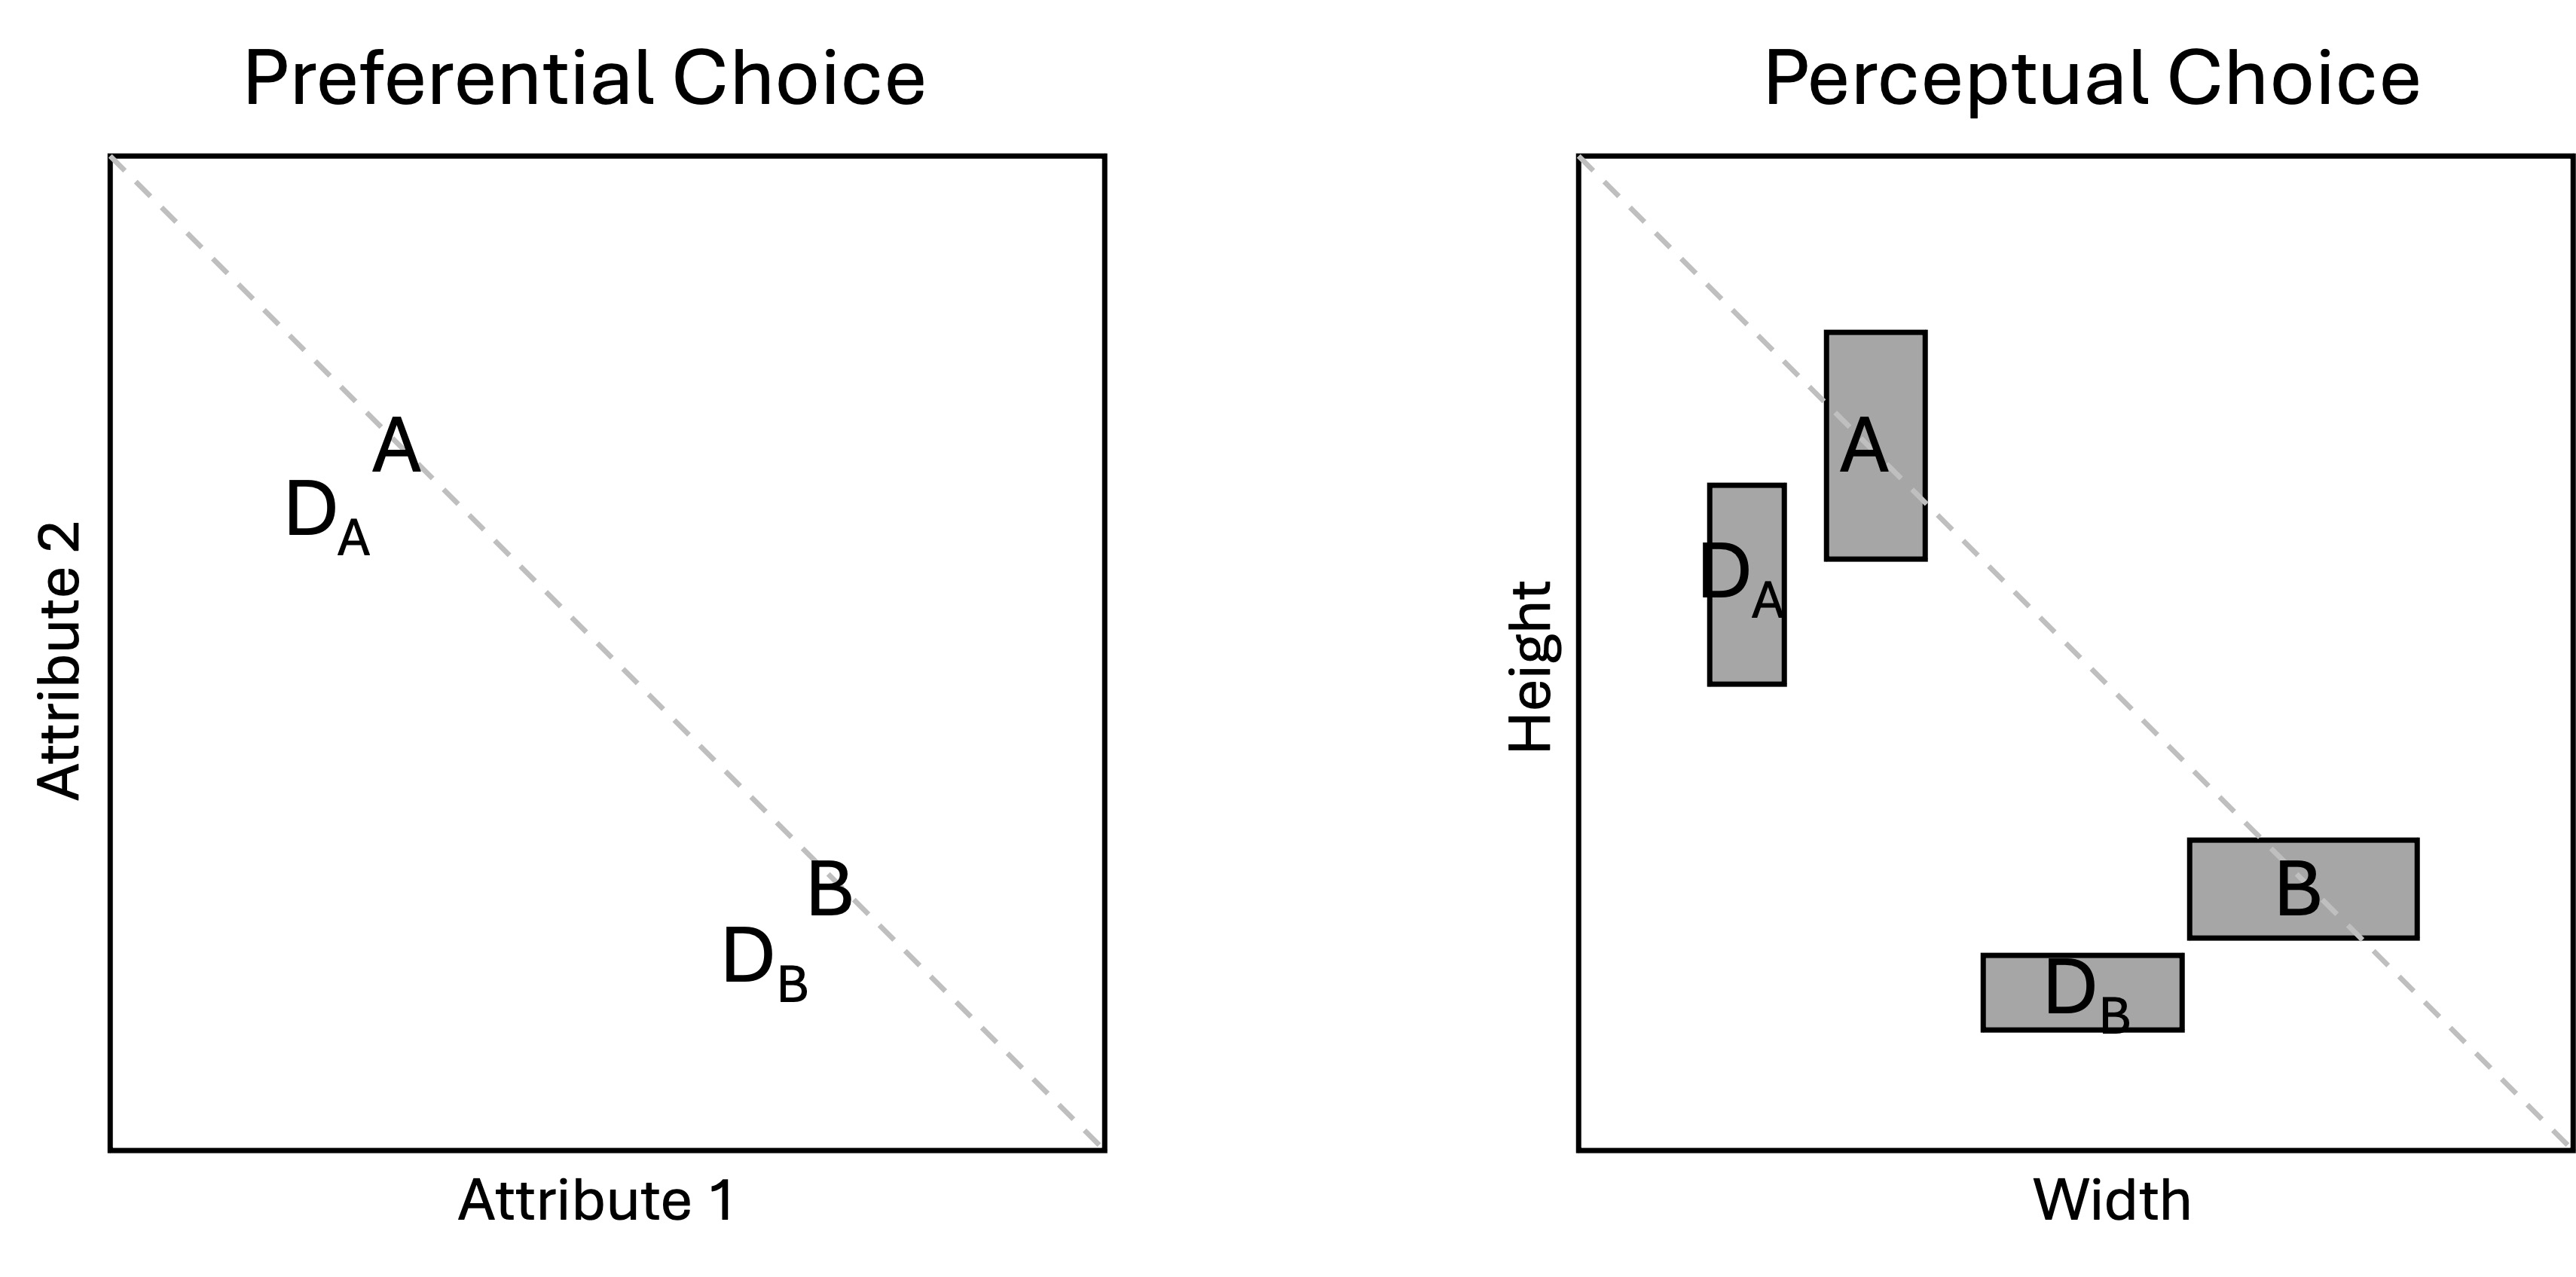
\includegraphics[width=\linewidth]{figures/pref_v_percep.jpg}
   \caption{A graphical depiction of choice options in the attraction/repulsion effect. Left panel: preferential choice. Right panel: perceptual choice.}
   \label{fig:fig_opts}
\end{figure}

To demonstrat IIAe, let $A$, $B$, $D_{A}$, and $D_{B}$ be discrete choice options, $[]$ denote the options in a choice set, and $P(A|[A,B])$ denote the probability of choosing option $A$ from a set consisting of $A$ and $B$. According to IIA:

\begin{align}
  \frac{P(A|[A,B,D_{A}])}{P(B|[A,B,D_{A}]}=\frac{P(A|[A,B,D_{B}])}{P(B|[A,B,D_{B}]}
  \label{eqn:iia}
\end{align}

However, in the attraction effect:

\begin{align}
  \frac{P(A|[A,B,D_{A}])}{P(B|[A,B,D_{A}]}>\frac{P(A|[A,B,D_{B}])}{P(B|[A,B,D_{B}]}
  \label{eqn:iia_att}
\end{align}

Thus, IIA is violated.

In the context effects literature, it is common to refer to the similar, dominated option as \textit{decoy}, the similar dominating option as a \textit{target}, and the dissimilar dominating option as a \textit{competitor}. I adopt this terminology through this dissertation. For example, in the choice set $[A,B,D_{A}]$, $A$ is the target, $B$ is the competitor, and $D_{A}$ is the decoy.  The decoy is dominated by the target, so no rational agent should intentionally select it over the target.  

The attraction effect was first demonstrated by \textcite{huberAddingAsymmetricallyDominated1982d} \footnote{These authors referred to this finding as the asymmetric dominance effect. To stay consistent with contemporary research, I use the term attraction effect throughout this dissertation.}, who tested participants with duples and triples of choice options, using products such as cars, beers, and TV sets. The authors showed that the introduction of an asymmetrically dominated decoy tended to increase the choice share of a similar, target option. Such a result violates IIA but also a principle known as regularity, which states that the introduction of another option to a choice set cannot increase the probability of choosing any given option (CITE COLONIUS 1984, MACKAY AND ZINNES 1995, MARLEY 1989). That is to say:

\begin{align}
  P(A|[A,B])\geqP(A|A,B.D_{A})
  \label{eqn:reg_att}
\end{align}

Thus, \textcite{huberAddingAsymmetricallyDominated1982d}'s finding that $P(A|[A,B])\leqP(A|A,B.D_{A})$ violates this assumption. \textcite{huber1983market} replicated these results and also showed that if the decoy has a relatively high value, it can actually take choice shares away from the target. This result suggests that the relative positioning of the decoy to the target can greatly affect patterns of choice, a finding explored by numerous other researchers which has strong theoretical consequences (see below). 

Numerous researchers have since demonstrated the attraction effect in preferential choice, including in real-world scenarios. \textcite{doyleRobustnessAsymmetricallyDominated1999} found an attraction effect in real world supermarket choices by adding a decoy option to an existing product set, where the decoy option was the same brand and price as the target, but of a lower volume. \textcite{van2021attract} showed that the attraction effect can be used to induce people to choose healthier food items. \textcite{slaughterDecoyEffectsAttributelevel1999b} showed that the attraction effect can be found even without the explicit attribute descriptions commonly used in laboratory experiments, when participants must infer option attributes. 

Context effects like the attraction effect have strong theoretical implications. Traditional models of choice, as used in economics and marketing research \parencite{mcfadden2001economic}, treat the \textit{utility}, or value, of each option as a random variable whose parameters are to be estimated from choice data, and on each trial of a choice experiment the participant samples values from these distribution and deterministically chooses the option with the highest sampled value. These models are known as \textit{Random Utility Models} (RUMs). When utilities are assumed to follow Type 1 Generalized Extreme Value distribution, the logit or softmax model is used (CITE). As will be the focus of much of this dissertation, the probit model assumes Gaussian distributed utilities (CITE). Often (though not necessarily) RUMs assume IIA, though this assumption can be relaxed by assuming set or alternative specific intercepts (CITE) or allowing correlations between options and/or attributes (CITE). \textcite{haaijer1998utility} showed that the probit model shows an improved fit to context effect data by allowing such correlations. I elaborate on this class of models below. 

In cognitive psychology, researchers have developed cognitive process models that attempt to explain the cognitive processes that lead to context effects \parencite{truebloodMultiattributeLinearBallistic,roeMultialternativeDecisionField2001a,usherLossAversionInhibition2004a,bhatiaAssociationsAccumulationPreference2013b,noguchiMultialternativeDecisionSampling2018a,wollschlager2NaryChoiceTree2012a,bergnerVAMPVotingAgent2019b,tverskyEliminationAspectsTheory1972,tversky1993context}. These models differ, to varying degrees, in their explanations for the attraction effect. Many, however, rely on comparisons between the target and the similar, but inferior, decoy, which boost an internal  preference state for the target. \textcite{roeMultialternativeDecisionField2001a}'s Multialternative Decision Field Theory (MDFT) model proposes that the similarity between target and decoy causes frequent target-decoy comparisons, and through a lateral inhibition, the negative valence for the decoy causes a boost to the preference state of the target at the expense of the competitor. \textcite{truebloodMultiattributeLinearBallistic}'s Multiattribute Linear Ballistic Accumulator (MLBA) model proposes that pairwise attention weights, which are a function of the similarity between options, increase the importance of target-decoy comparisons and thus boost preference for the target. 

This dissertation does not explore the predictive success of these models, nor does it incorporate model fitting to compare these models. Indeed, other researchers have done such analyses \parencite{turnerCompetingTheoriesMultialternative2018a,cataldoModelingPreferenceReversals2021,evansResponsetimeDataProvide2019b,molloyWhatResponseTime2019a,berkowitschRigorouslyTestingMultialternative2014b}. Instead, I use behavioral experiments and statistical modeling to understand how context dependence arises in various domains.

The attraction effect is not limited to merely consumer choice. Researchers have found the attraction effect in risky choice \parencite{mohr2017attraction}, policy choice \parencite{herneDecoyAlternativesPolicy1997b}, intertemporal choice \parencite{mariniAttractionComesMany2020}, probability judgment \parencite{caiWhenAlternativeHypotheses2023}, medical decision-making \parencite{schwartz1999more}, charitable donation \parencite{pittarello2020three},  inference \parencite{truebloodMultialternativeContextEffects2012}, job candidate selection \parencite{highhouseContextDependentSelectionEffects1996}, political choice \parencite{pan1995attractiovoting}, and, as will be the focus of much of this dissertation, perceptual choice \parencite{evansImpactPresentationOrder2021,trueblood2013not,spektorRepulsionEffectPreferential2022,spektorWhenGoodLooks2018b,yearsleyContextEffectsSimilarity2022,turnerCompetingTheoriesMultialternative2018a,liaoInfluenceDistanceDecoy2021}. 

\subsection{From preferential to perceptual choice}

As mentioned above, researchers have begun studying context effects in perceptual choice. \textcite{trueblood2013not} demonstrated the attraction effect in perceptual choice. In their experiments, participants saw three rectangles on each trial, arranged in a horizontal array, and they selected the option they believed to have the largest area. As a demonstration of this stimulus configuration, see \ref{fig:fig_opts} (right panel).  Options $A$ and $B$ have equal area but trade off in height and width. \footnote{\textcite{trueblood2013not} also demonstrated the similarity and compromise effects.} Notably, the title of their paper was "Not Just for Consumers: Context Effects Are Fundamental to Decision Making", and in their General Discussion, \textcite{trueblood2013not} argued "our experiments suggest that these context effects are a general feature of human choice behavior because they are a fundamental part of decision-making processes. As such, our results challenge explanations of these effects exclusively in terms that are unique to high-level decision making and thus call for a common theoretical explanation that applies across paradigms." (p. 907). According to \textcite{trueblood2013not}, context effects are not idiosyncratic to high-level choices but are a fundamental part of the choice process. \textcite{trueblood2013not} also used these perceptual results to argue against the context-dependent advantage (CDA) model developed by \textcite{tversky1993context} as well as the Leaky Competing Accumulators model of \textcite{usherLossAversionInhibition2004a}, as these models use "loss aversion" (i.e., the idea that an option's disadvantages on an attribute are weighted more strongly than its advantages on other attributes) to account for context effects. 

\textcite{turnerCompetingTheoriesMultialternative2018a} replicated \textcite{trueblood2013not}'s results and performed a large scale modeling study. The authors compared the ability of numerous mechanisms assumed by decision models to account for context effects. For example, \textcite{turnerCompetingTheoriesMultialternative2018a} concluded that pairwise comparisons on individual attributes greatly improves models' ability to account for context effects. This may not be appropriate, however, given a perceptual domain where dimensions may not be separable \parencite{ashbyVarietiesPerceptualIndependence1986a}. 

\textcite{spektorWhenGoodLooks2018b} followed up on this work and demonstrated the \textit{repulsion effect} in a rectangle choice experiment. In the repulsion effect, the competitor's choice share is higher than the target's choice share \parencite{liaoInfluenceDistanceDecoy2021,evansImpactPresentationOrder2021,simonsonVicesVirtuesMisguided2014,frederickLimitsAttraction2014b,spektorRepulsionEffectPreferential2022,banerjeeFactorsThatPromote2024,bhui2021rational}. In \textcite{spektorWhenGoodLooks2018b}'s experiments, the target and competitor options varied in area, such that one option was always larger, but on average they were the same size. The researchers also varied the \textit{target-decoy attribute distance} (TDD), the percentage difference between the target and decoy areas. For example, if TDD is $2\%$, the decoy is $2\%$ smaller than the target. 

\begin{figure}
   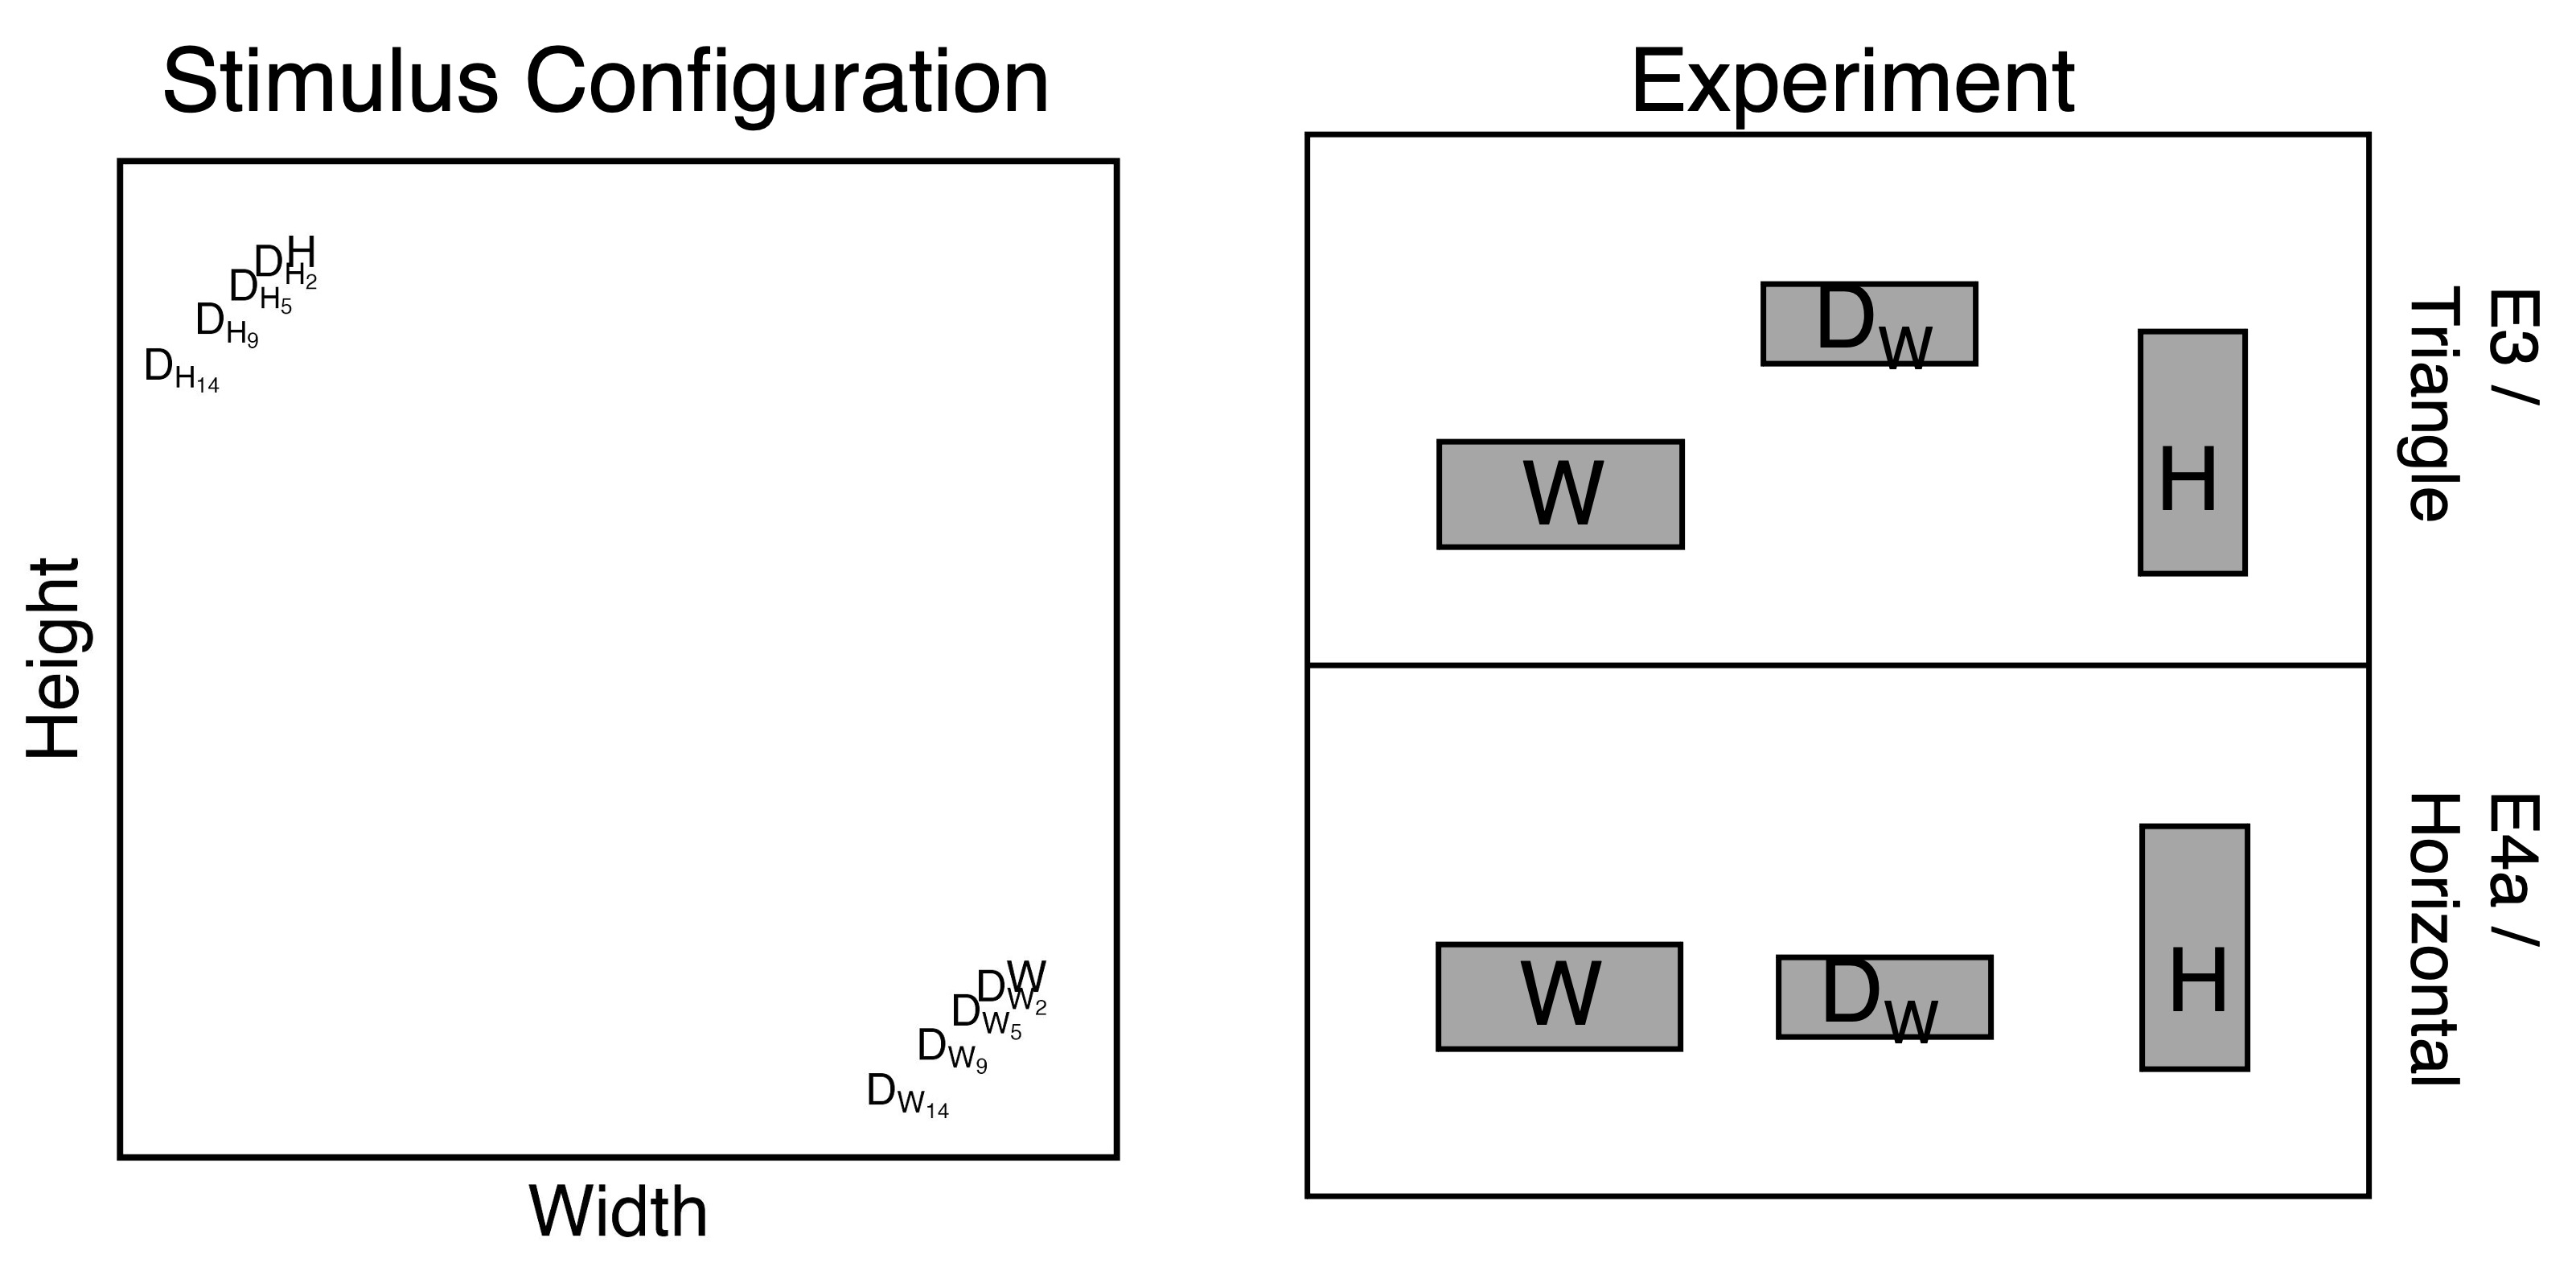
\includegraphics[width=\linewidth]{figures/spektor_stim.png}
   \caption{Stimulus configuration and example trials from \textcite{spektorWhenGoodLooks2018b}, Experiments 3 and 4a.}
   \label{fig:spektor_stim}
\end{figure}

\textcite{spektorWhenGoodLooks2018b} ran a total of five experiments, but I focus on their experiments 3 and 4a here. In Experiment 3, the authors varied TDD at four levels: $2\%$, $5\%$, $9\%$, and $14\%$. The rectangles were arranged in a trianglular display on the screen (see Figure \ref{fig:spektor_stim}, Experiment 3), in contrast to \textcite{trueblood2013not}'s horizontal display. \textcite{spektorWhenGoodLooks2018b} found an empirical repulsion effect such that the competitor was selected more than the target at all levels of TDD (see Figure \ref{fig:spektor_stim}). 

\textcite{spektorWhenGoodLooks2018b} also ran a follow-up experiment using the horizontal diplay of \textcite{trueblood2013not} (see Figure \ref{fig:spektor_stim}, Experiment 4a). Here, they varied TDD at $5\%$, $9\%$, and $14\%$. In Experiment 4a, the data show a slight repulsion effect at low TDD levels that eventually becomes an attraction effect at high TDD levels. 

\begin{figure}
   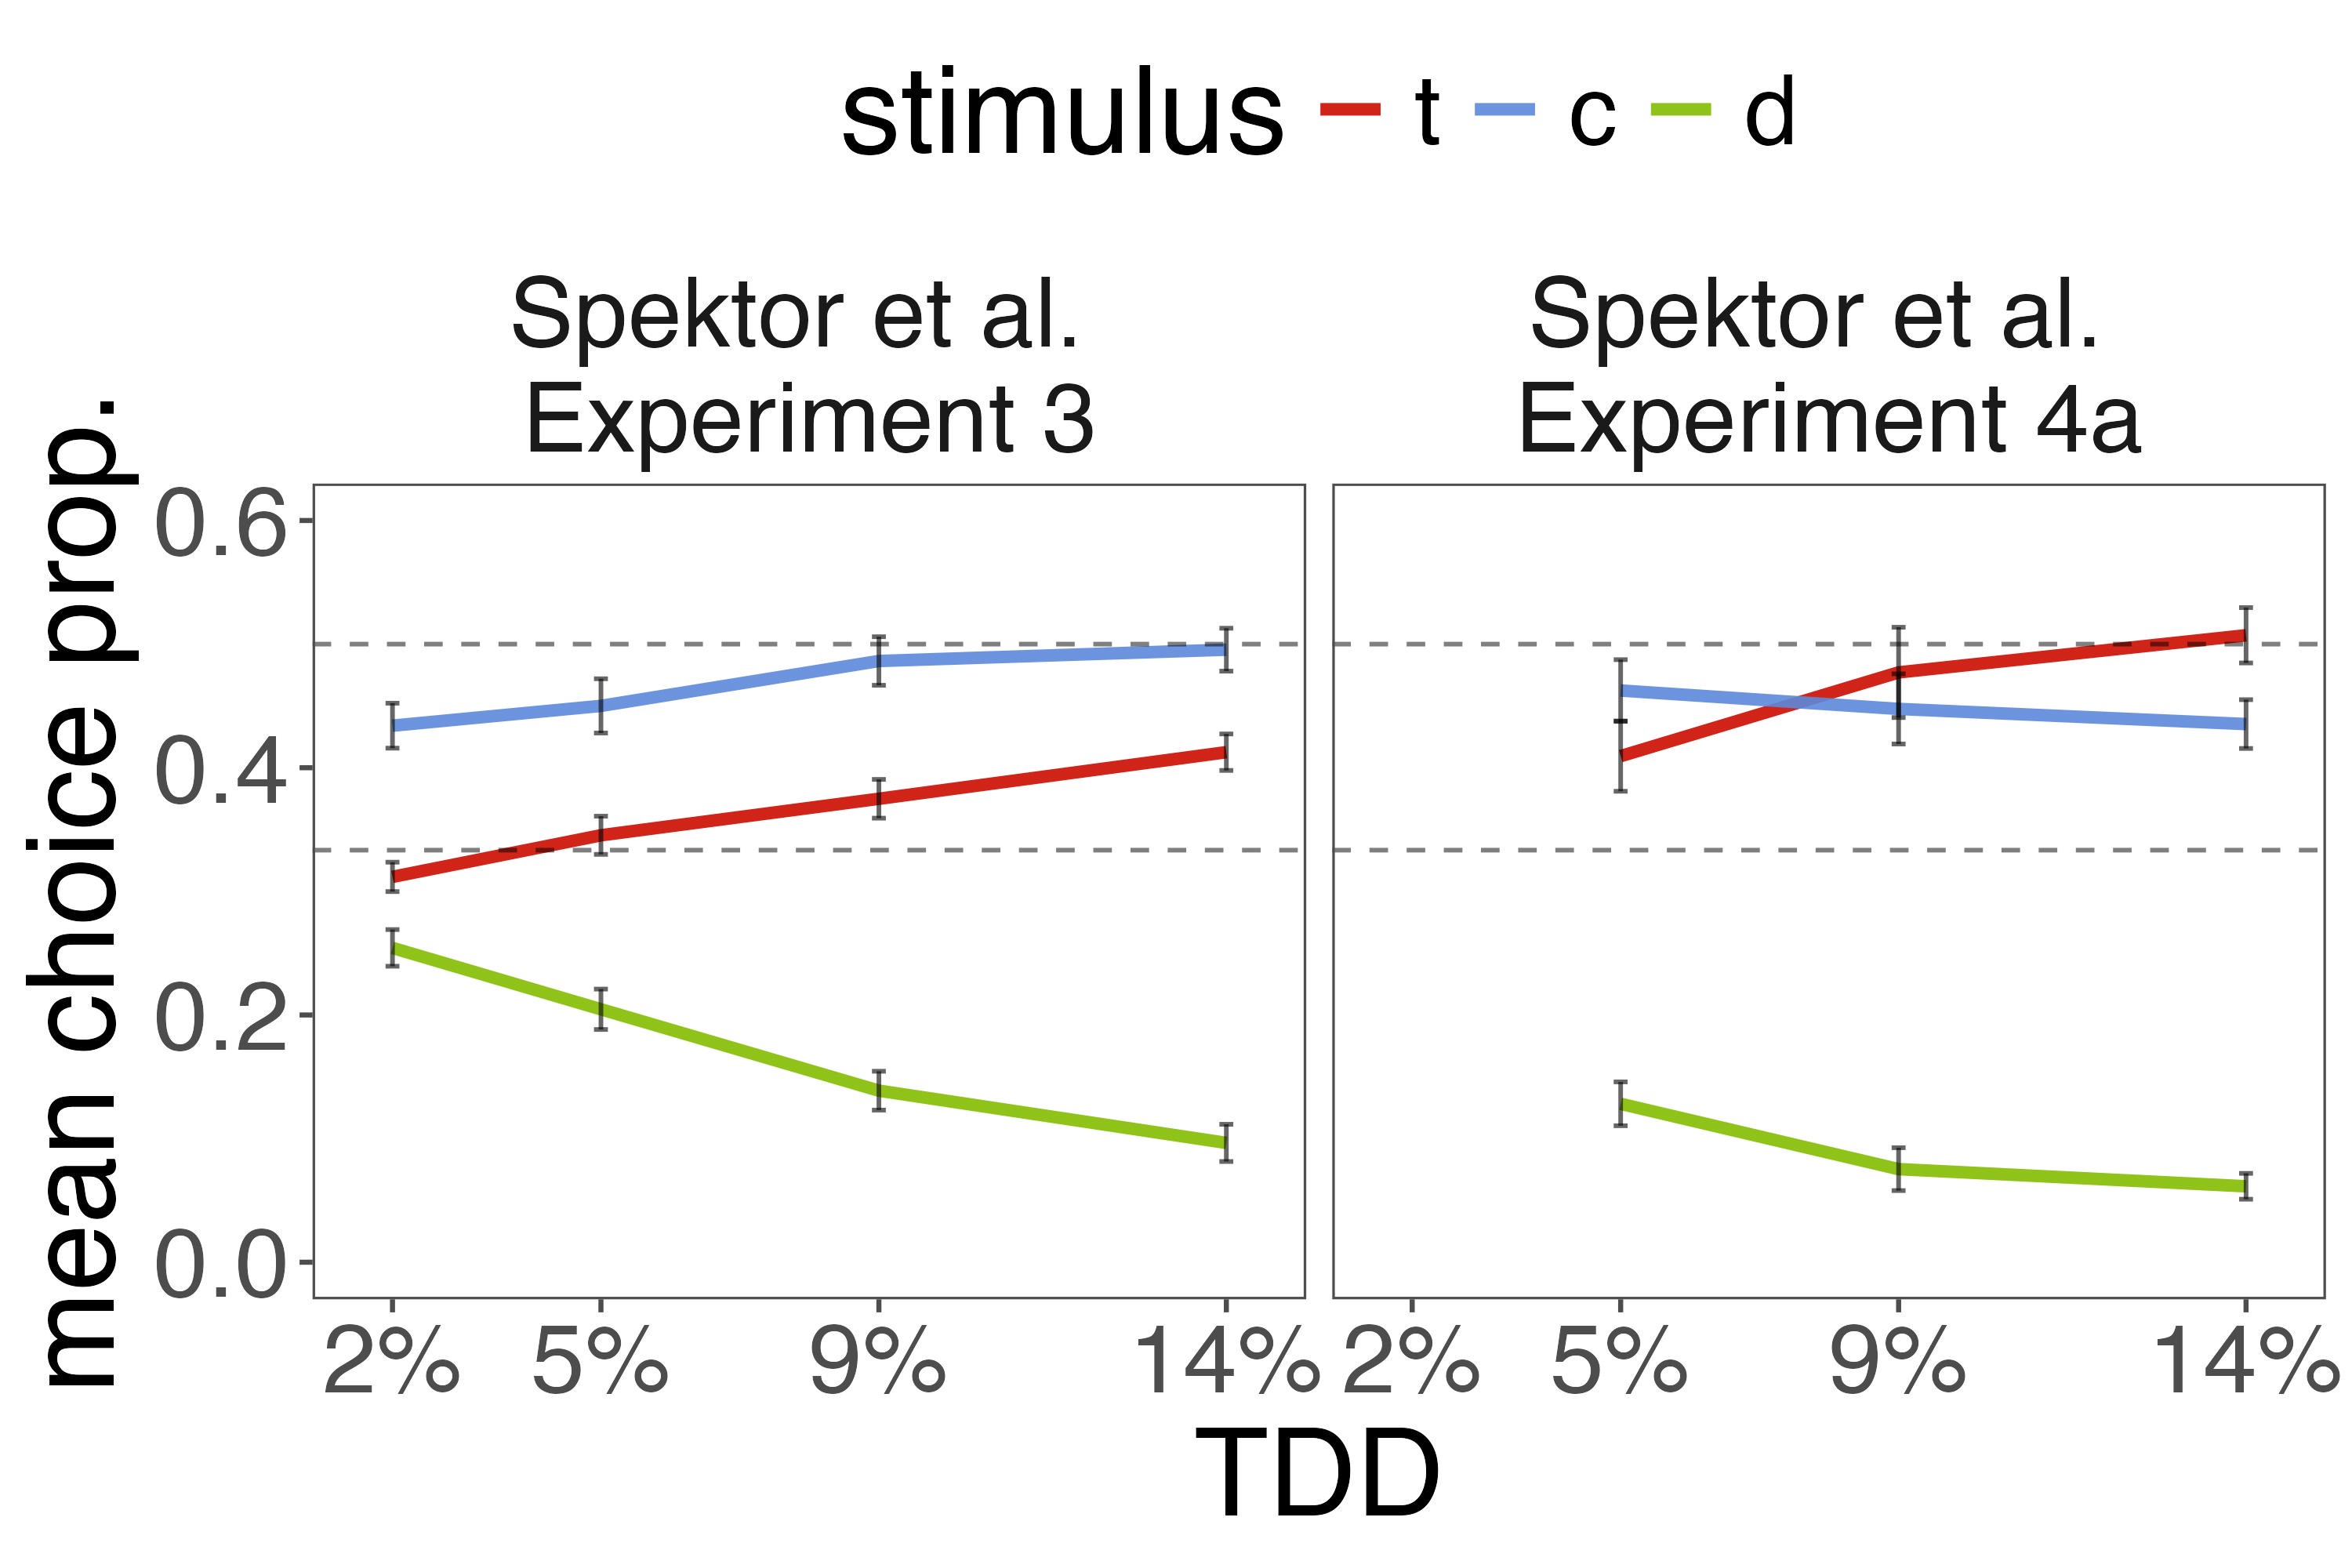
\includegraphics[width=\linewidth]{figures/spektor_data_collapsed.jpeg}
   \caption{Data from \textcite{spektorWhenGoodLooks2018b}, collapsed across choice set. Error bars are $95\%$ CIs of the mean, computed using the within-subjects error correction from \textcite{morey2008confidence}. Dashed lines are drawn at .5 and .33.}
   \label{fig:spektor_data} % might consider graphing (or at least writing RSTs) here
\end{figure}

\textcite{liaoInfluenceDistanceDecoy2021} also replicated the general pattern of \textcite{spektorWhenGoodLooks2018b}'s results and also found a an inverse U-shaped relationship between TDD and RST\footnote{$RST=\frac{P(T|[T,C,D])}{P(T|[T,C,D)+P(C|[T,C,D])}$}. Relatively low and extremely high TDD values created a repulsion effect, while intermediate TDD values created an attraction effect. 

\textcite{spektorRepulsionEffectPreferential2022} demonstrated the repulsion effect in both preferential and perceptual choice, using similar stimuli and display configuration. In these experiments, each stimulus option contained a square with two partially filled bars. In perceptual choice, participants were to select the stimulus with the largest cumulative filled area. In the preferential choice scenario, participants were told that each filled bar represented one possible outcome of a 50-50 gamble, and they were to select the gamble with the highest expected value. Their results were similar to those of \textcite{spektorWhenGoodLooks2018b}, however, where target and competitor choices increased with TDD, with target and decoy showing a particularly strong trade-off.

Researchers are clearly using perceptual experiments to demonstrate context effects and test theory. These results are clearly informative and theoretically interesting. I argue, however, that researchers should be cautious in assuming that decision-makers receive perceptual input with the same accuracy that they do in preferential choice experiments. Researchers should seek to separate the role of perceptual discriminability from decisional processes when understanding participants' responses. I elaborate on these ideas below, with a demonstration using the results of \textcite{spektorWhenGoodLooks2018b}.

\subsection{Understanding Perceptual Choice Experiments}

I seek to understand the role of perception in perceptual choice context effect experiments. To do so, I take an extreme stance - that such experiments are solely perceptual experiments rather than decision-making experiments and that no high level decision processes are occurring. This extreme assumption is incorrect, but I believe it is a good place to start in understanding existing data. I also demonstrate how and under what circumstances it is incorrect later in this dissertation. To begin, I return the results of \textcite{spektorWhenGoodLooks2018b}. 

As reported above, \textcite{spektorWhenGoodLooks2018b} demonstrate that a relatively small change in stimulus display (arranging stimuli in a triangle rather than a horizontal line) reverses the attraction effect. Why is this? To begin to answer this question, I highlight the differences between \textcite{spektorWhenGoodLooks2018b}'s data and previous context effect data. In preferential choice tasks, participants are given a set of options on each trial (e.g., laptops, apartments, washing machines), along with the attribute values associated with each option (e.g., 10 GB RAM, 1500 square feet, 2.7 cubic feet capacity). These attributes are typically represented numerically \parencite{hayes2024attribute,banerjeeFactorsThatPromote2024} or with easily discriminable graphical representations \parencite{cataldoComparisonProcessAccount2019b}. The decoy option, therefore, is rarely selected (e.g., $<5\%$ of all trials), and these selections are assumed to be the result of inattention or accidental responses. Researchers assume that participants are able to detect the dominance relationship between target and decoy. Perceptual choice tasks complicate participants' ability to detect this dominance relationship. In \textcite{spektorWhenGoodLooks2018b}'s experiments, the decoy is selected as often as $25\%$ of all trials in some conditions. The decoy is selected less often in experiment 4a (triangle display) than in experiment 3 (horizontal display). Decoy selections also decrease as the difference between decoy area and target/competitor areas increases. Finally, though both target and competitor increase in choice share as TDD increases, the target choice share increases at a higher rate than does the competitor, suggesting a strong trade-off between target and decoy choices (stronger, indeed, than that of competitor-decoy choices). That is, the mean \textit{Relative Share of the Target} (RST) \parencite{berkowitschRigorouslyTestingMultialternative2014b} increases with TDD in both experiments % should I explicitly show or write mean RST values? -Sean 1/9/25

Clearly, perceptual discriminability plays a role in \textcite{spektorWhenGoodLooks2018b}'s results. Participants clearly are better able to discriminate the target and competitor from the decoy as the decoy decreases in size. Any reasonable account of these data should parse the out discriminability from genuine context effects. 

There is a large body of psychological research, beginning with the work of \textcite{thurstone1927law}, of treating the perception of a stimulus as a random variable. In his famous "Law of Comparative Judgment" paper, \textcite{thurstone1927law} first showed that researchers can use binary choice proportions to estimate the psychological distance between stimuli, by treating perceptual intensity as a Gaussian random variable. This work led to similar research using Signal Detection Theory (STD) \parencite{hautus2021detection}, which also treats psychological quantities (e.g., memory, perception), as random variables. Similarly, Ashby and colleagues' General Recognition Theory (GRT) models the perception of a stimulus as a multivariate normal random variable, where each dimension of the model is the perceived dimension of a stimulus \parencite{ashbyVarietiesPerceptualIndependence1986a,ashby1988decision, ashbyUnifiedTheorySimilarity}. In marketing and economics, researchers treat the utilities of choice options as random variables, which are often assumed to be Gaussian or Extreme Value Distributed and estimate choice models known as Random Utility Models \parencite[RUMs,]{mcfadden2001economic,hausman1978conditional,train2009discrete}.Often, though not necessarily, these models share the common property that value (whether it is the utility of a consumer product, the perception of magnitude, or the memory signal in a recognition task) is stochastic while choice is deterministic \parencite[c.f.,]{benjamin2009signal} I consider this class of models throughout this paper.
